\chapter{Developed Tools}

This chapter contains an overview of why supplementary tools were deemed necessary for an already working reduction process (\S~\ref{sec:polsalt_limits}), which aspects of the reduction process have been altered, replaced, or added (\S~\ref{sec:mod_tools}, \ref{sec:add_tools}), and finally what an updated reduction process consists of using a combination of all software (\S~\ref{sec:red_proc}).


\section{Limitations of POLSALT and the Need for a Supplementary Tool} \label{sec:polsalt_limits} % Rename

% Why
The creation of supplementary tools for \textsc{polsalt} spectropolarimetric reductions stem from, primarily, the limitations of the wavelength calibration process and a need for a way to compare wavelength solutions across matching $O$ and $E$ polarization beams. Due to the time-consuming process of recalibrating the wavelength solutions it is not feasible to perform the wavelength calibrations time and time again for any amount of reductions larger than a handful of observations.
\prgph

% How
One solution is to use a well established tool to perform the wavelength calibration, one which allows for rapid recalibrations as well as provides a familiar interface with which the user can analyze their wavelength solutions. \textsc{iraf} provides this familiar environment and reliability, even considering it's age and \hyperlink{https://github.com/iraf-community/iraf}{limited community development}. Unfortunately, \textsc{iraf} is unable to parse the file structure implemented by \textsc{polsalt} as is and formatting of the data structures are necessary for integration purposes. This restructuring works both ways as once the \textsc{iraf} reductions are complete the format must be reformatted to match that of the \textsc{polsalt} output such that the reduction process may carry on in \textsc{polsalt}.
\prgph

\todo{The main takeaway should be the need for a way to do the wavelength calibration with more control as well as the need to check the O/E beam wavelength calibrations against one another (since very accurate wavelength calibration necessary for stokes parameter calculations). Feels like something is missing in this section.? Mention difficulty with PG0300? Mention GUI difficulties?}


\section{Wavelength calibrations using the Supplementary Pipeline and IRAF} \label{sec:mod_tools}

The supplementary tools offer an alternate procedure for wavelength calibrations for the \textsc{polsalt} pipeline. This procedure can be broken into three unique steps: the parsing of \textsc{polsalt} data into an \textsc{iraf} friendly format, from here on referred to as splitting; the wavelength calibration performed in \textsc{iraf}; and the reformatting of the data with its wavelength calibration back into the format expected by \textsc{polsalt}, from here on referred to as joining.

\begin{figure}[t]
    \centering
    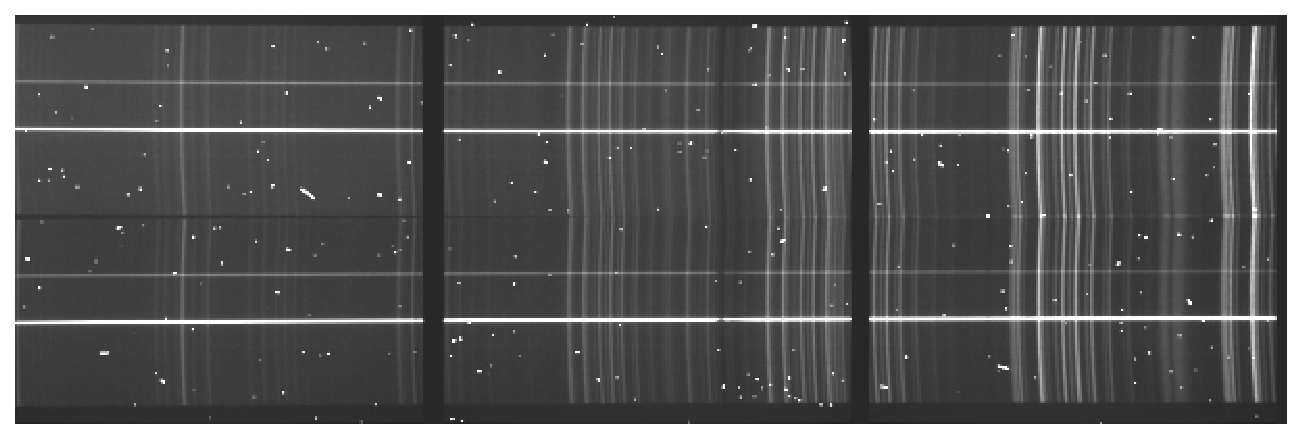
\includegraphics[width = 1.0\textwidth]{figures/3_pre_wav_cal.pdf}
    \caption{The science extension of a typical \textsc{polsalt} \gls{FITS} file after basic \gls{CCD} reductions have been completed.}
    \label{fig:polsalt_pre_wav_cal}
\end{figure}


\subsection{Splitting the POLSALT pre-calibration files}

% Why necessary
%   Mention steps before and how they return (especially) the file structure.
As mentioned previously, the format of the \gls{FITS} file created by \textsc{polsalt} after basic \gls{CCD} reductions and that expected by \textsc{iraf} to be used for the wavelength calibrations are incompatible. A typical \gls{FITS} file created by the \textsc{polsalt} basic \gls{CCD} reductions process contains a primary header along with the various image extensions, all of which include the trace for both polarimetry beams, as seen in Figure~\ref{fig:polsalt_pre_wav_cal}. \textsc{iraf} deals best with a singular trace, and therefore a singular polarization beam, at a time.
\prgph

In an attempt to simplify the \textsc{iraf} reduction procedure it was decided to split the polarization beams into their own files, as the parameters of \textsc{iraf} tasks generally handle lists of files better than subregions of the same \gls{HDU}, and generally allowed for easier calibrations further down the \textsc{iraf} wavelength calibration process.
\prgph

% What it does -> Primary focus
%   All processes run & description of each. Focus on why.
The \textsc{polsalt} files with basic \gls{CCD} reductions applied, namely \gls{FITS} files with the prefix `mxgbp' (\S~\ref{subsec:polsalt}), are used as the starting point for the supplementary tool's splitting method. Running the split method finds all the \gls{FITS} files for wavelength calibration within the working directory, creates two empty \gls{HDU} structures for each sub-extension of the \gls{FITS} file, and appends all science and header data necessary for wavelength calibration to the relevant \gls{HDU} structure.
\prgph

% Focus on minimizing changes and optimizing size
As the intent was always to parse the wavelength function back into \textsc{polsalt} it was decided to keep these temporary \gls{FITS} files as light as possible. This is especially necessary when considering the amount of frames that must be taken for a single spectropolarimetric observation, and then how that increases for long term studies.
\prgph

\begin{figure}[t]
    \centering
    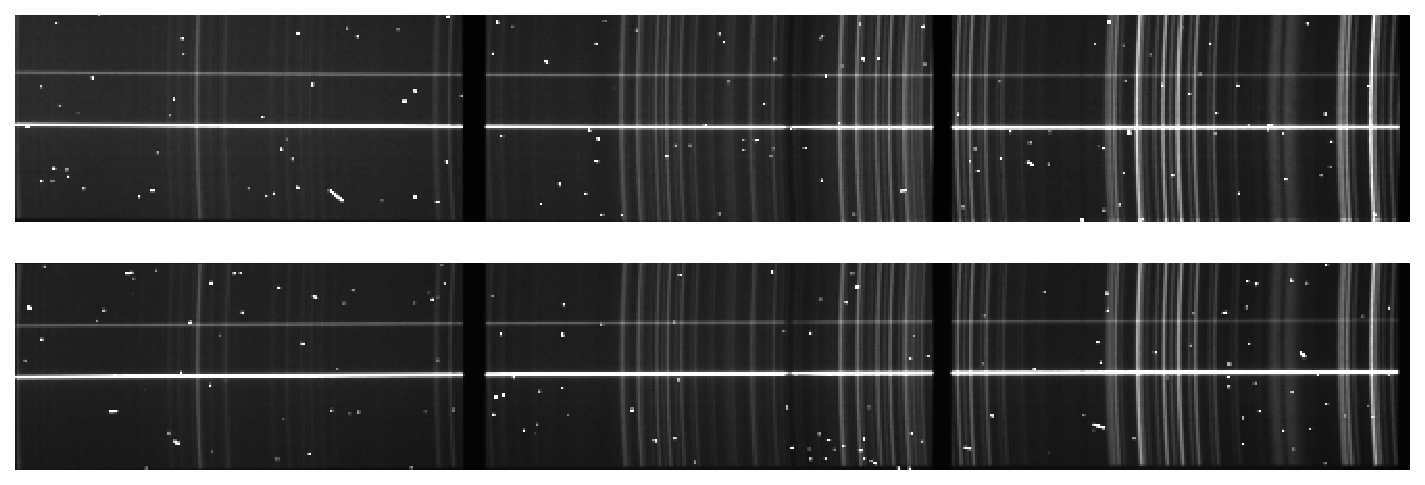
\includegraphics[width = 1.0\textwidth]{figures/3_OEsplit.pdf}
    \caption{The split $O$ and $E$ beams as handed to \textsc{iraf}.}
    \label{fig:OE_split}
\end{figure}

% Any changes from how polsalt would do it
In an attempt to automate the scripting of the \textsc{iraf} wavelength calibrations, row cropping was introduced into the split method to ignore the regions without a trace either side of the frame, and the creation of files listing the $O$ and $E$ beams. The row cropping was decided on as \textsc{iraf} does not handle the empty rows well, specifically when it comes to the \textit{reidentify} task. Otherwise, defaults, such as which row to split the beams along, were kept as close to the \textsc{polsalt} pipeline as possible.


\subsection{IRAF wavelength calibration}\label{subsec:IRAF_wav_cal}

% Why necessary
As every university and research group has their own preferred wavelength calibration procedure and often use certain parameters for the various \textsc{iraf} tasks, only a brief overview of the tasks used will be provided here.

% What it does -> Primary focus
%   All processes run & description of each. Focus on why.
\paragraph{Identify}
\todo{Description of identify task and why performed emphasis instead of how}
\prgph

\paragraph{Reidentify}
\todo{Description of reidentify task and why performed emphasis instead of how}
\prgph

\paragraph{Fitcoords}
\todo{Description of fitcoords task and why performed emphasis instead of how}
\prgph

\paragraph{Transform}
\todo{Description of transform task and why performed emphasis instead of how}
\todo{Mention optional, good for sanity checks which is not possible using the pure polsalt implementation}
\prgph

% Files created and/or modified
\todo{Files created or modified throughout the wavelength calibration process.}

\subsection{Joining the wavelength calibrated files}

\todo{
    \begin{itemize}
        \item Load files and wavelength functions
        \item create empty hdu
        \item update headers
        \item copy data
        \item append new extensions
        \item parse and save wavelength functions as image
        \item cosmic ray cleaning
        \item polsalt specific cropping (wav mask)
        \item mask wavelength using wollaston curve for polsalt `parsability'
        \item update BPM to reflect wavelength cropping
    \end{itemize}}

\todo{Return file structuring.}
\prgph

\todo{Focus on \textbf{why}. Parsing \textsc{iraf} frames to be used by POLSALT and making sure the header and extensions reflect the changes}

\begin{figure}[t]
    \centering
    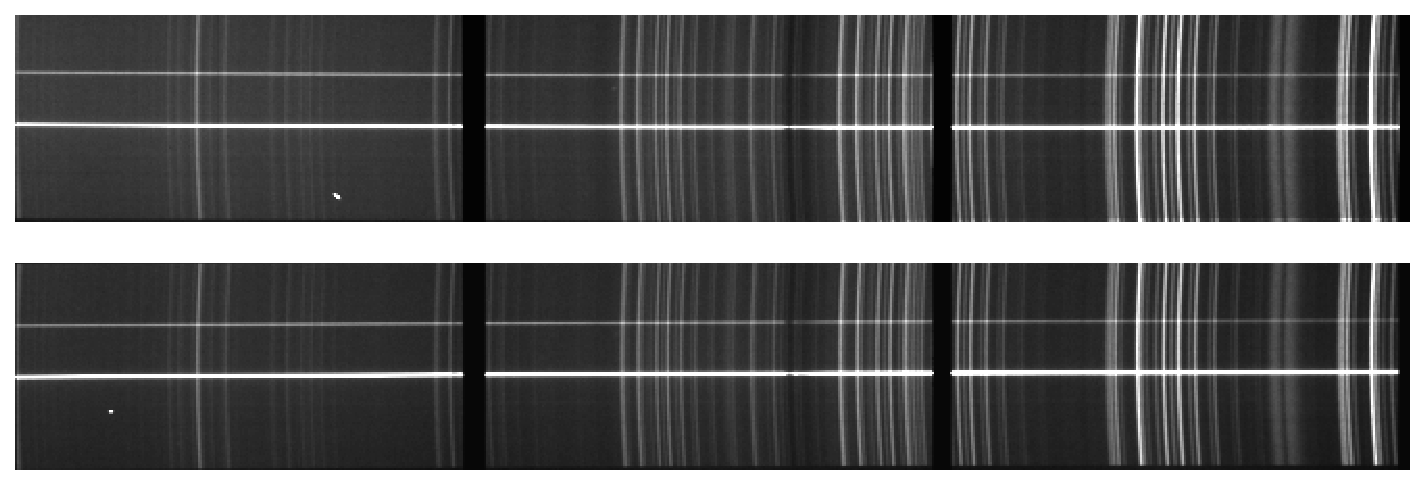
\includegraphics[width = 1.0\textwidth]{figures/3_post_wav_cal.pdf}
    \caption{The science extension of a \gls{FITS} file ready to be handed back to the \textsc{polsalt} pipeline.}
    \label{fig:polsalt_post_wav_cal}
\end{figure}


\section{Additional Tools}\label{sec:add_tools}

Along with the ability to perform wavelength calibrations in \textsc{iraf}, it was deemed necessary to create tools to allow for the comparison of the $O$ and $E$ beams.

\todo{fill out}

\subsection{Cross correlation}

\todo{Why a cross correlation necessary and how it works}


\subsection{Skyline comparisons}

\todo{REMOVE? Not truly implemented... Again, why a skyline comparison necessary and how it works. Also, how the frame is transformed (\textsc{iraf} bypassed) and that the flux is not conserved so only for checking and not for science use.}


\section{General Reduction Procedure}\label{sec:red_proc}

\begin{figure}[t]
    \centering
    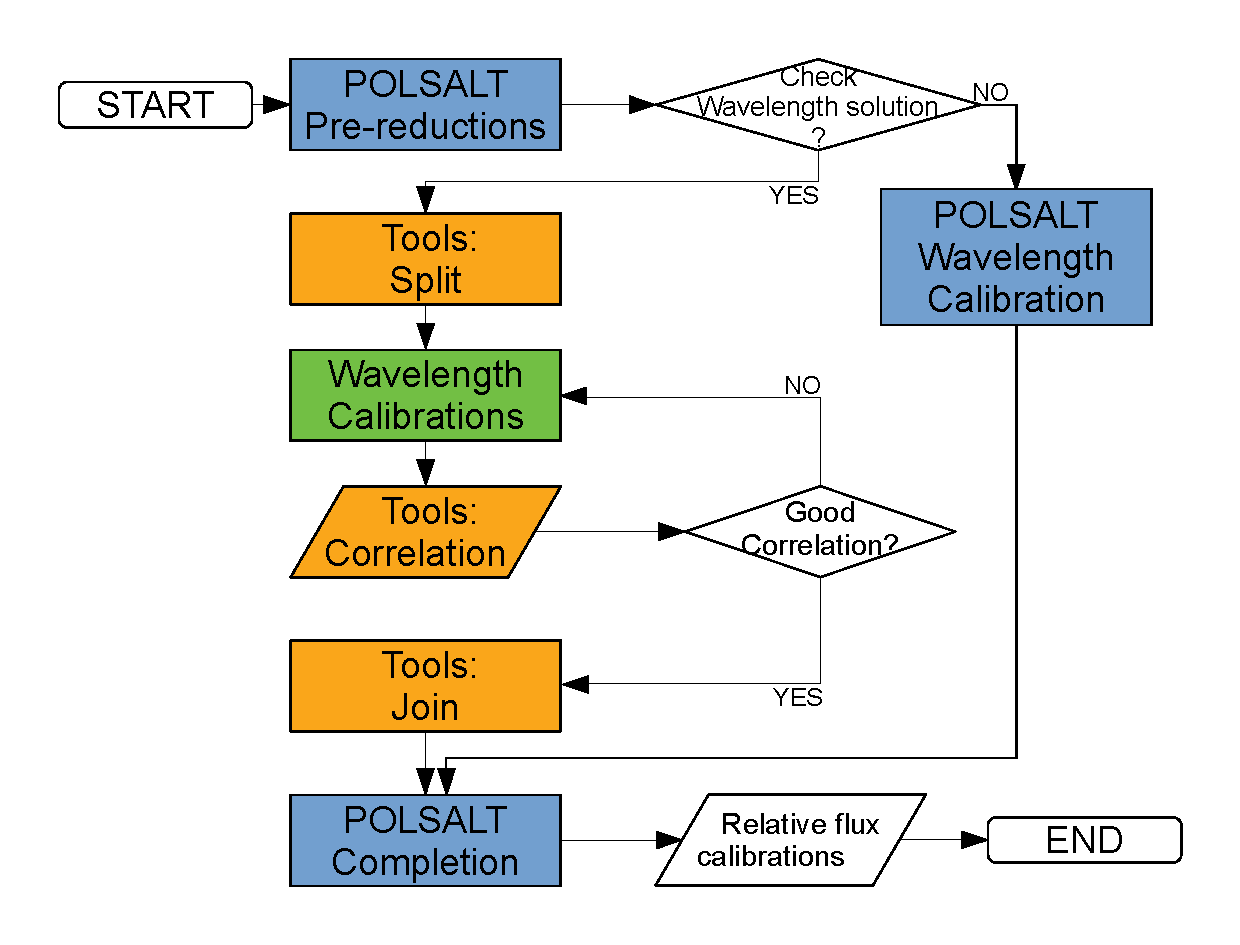
\includegraphics[width = 0.7\textwidth]{figures/3_new_workflow.pdf}
    \caption{A general workflow for data reductions using a combination of \textsc{polsalt}, \textsc{iraf}, and the developed supplementary tools.}
    \label{fig:new_workflow}
\end{figure}

\todo{General reduction procedure from raw data to finalized results
    \begin{itemize}
        \item This includes \textsc{polsalt} pre-reductions, splitting, \textsc{iraf} wavelength calibrations, checking, joining, and \textsc{polsalt} finalization. (Include Relative flux calibrations for `shape correcting' spectrum??)
    \end{itemize}
}